%!TEX root = ../main.tex
\section{Linear Systems, Linear Feedback}
\label{sec:lqg}

We start with the linear–quadratic regulator problem with a Gaussian linear policy (LQG). Dynamics and reward are:
\begin{subequations}\label{eq:lqr-dynamics-reward}
\begin{align}
  s_{t+1} &= A s_t + B a_t,\quad s_t\in\mathbb{R}^n,\ a_t\in\mathbb{R}^m, \\
  r(s,a) &= -\big(s^\top Q_s s + a^\top Q_a a\big),\quad Q_s, Q_a \succeq 0.
\end{align}
\end{subequations}
Actions are sampled from a stochastic policy $\pi(a\mid s) \sim \mathcal{N}(K s, \Sigma)$ with $\Sigma \succ 0$, and the initial state satisfies $s_0\sim\mathcal N(0,\Sigma_0)$ with $\Sigma_0 \succeq 0$. The closed-loop dynamics of \eqref{eq:lqr-dynamics-reward} can be written as $s_{t+1} = F s_t + B \epsilon_t$, where $\epsilon_t \sim \mathcal{N}(0, \Sigma)$ and $F := A + BK$. We study the policy gradient and its REINFORCE estimator \wrt the gain matrix $K$ and the policy covariance $\Sigma=\text{diag}(\sigma)^2$, parameterized by the log-standard deviation (log-std) \(\ell=\log\sigma\in\mathbb R^m\).

\textbf{Outline.} In \S\ref{sec:one-step-lqg}, we derive closed-form expressions for one-step LQG and analyze scaling with the initial-state and policy covariances. In \S\ref{sec:multi-step-lqg}, we extend the analysis to multi-step LQG and provide an exact numerical procedure for computing the variance and NSR, along with an upper bound that reveals key scaling factors. In \S\ref{sec:lqg-experiment}, we visualize the NSR along optimization trajectories on a double-integrator example and discuss the observed behavior.
% \begin{itemize}
%   \item \textbf{Linear policy (LQG-style):}
%   \[
%     \mu_\theta(s)=K s,\qquad a_t \sim \mathcal N(K s_t,\ \Sigma).
%   \]
%   \item \textbf{Neural policy (MLP):}
%   \[
%     \mu_\theta(s)=\mathrm{MLP}(s),\qquad a_t \sim \mathcal N(\mu_\theta(s_t),\ \Sigma).
%   \]
% \end{itemize}

% With \(\gamma\in(0,1]\) and \(s_0\sim\mathcal N(0,\Sigma_0)\). We estimate the gradient of  \(\theta = K\); for the neural policy, \(\theta=\{W_i,b_i\}_i\).
% We also estimate gradients with respect to the covariance \(\Sigma\), parameterized via a log-standard-deviation. For simplicity, assume \(\Sigma\) is diagonal and denote its standard deviations by \(\sigma\in\mathbb R^m\) and log-stds by \(\ell=\log\sigma\in\mathbb R^m\).

% \subsection{Exact gradient}

% Let \(F:=A+BK\) and \(W:=B\Sigma B^\top\), with \(A,B,Q_s,Q_a\) as in \eqref{eq:lqr-dynamics-reward}. The state-covariance recursion is
% \[
% P_{0}=\Sigma_0,\qquad
% P_{t+1}=F P_t F^\top + W,\quad t=0,\dots,T-1 .
% \]

% \begin{theorem}[Finite-horizon analytical gradient]
% \label{thm:lqg-finite-gradient}
% With linear dynamics \eqref{eq:lqr-dynamics-reward}, the finite-horizon objective \eqref{eq:objective-definition} can be written as
% \begin{equation}
% \label{eq:lqr-objective-matrix-form}
% J_T(K,\Sigma)
% = -\sum_{t=0}^{T-1}\gamma^{t}\!\left(\tr(Q_s\,P_{t+1})
% +\tr(Q_a\,K P_t K^\top)+\tr(Q_a\Sigma)\right).
% \end{equation}
% Define the backward (adjoint) sequence $\{\Lambda_t\}_{t=0}^{T}$ by
% \begin{equation}
% \label{eq:lqr-lambda-rec}
% \Lambda_T=\tfrac{1}{\gamma}\,Q_s, \qquad
% \Lambda_t \;=\; \tfrac{1}{\gamma}\,Q_s \;+\; K^\top Q_a K \;+\; \gamma\,F^\top \Lambda_{t+1} F,
% \quad t=T-1,\dots,0.
% \end{equation}
% Then the gradient with respect to $K$ is
% \begin{equation}
% \label{eq:lqr-dJdK}
% \nabla_{K} J_T
% \;=\; -\,2\sum_{t=0}^{T-1}\gamma^{t}\Big( Q_a K P_t \;+\; \gamma\, B^\top \Lambda_{t+1} F\, P_t \Big)
% \;\in\; \mathbb{R}^{m\times n}.
% \end{equation}
% The gradient with respect to $\Sigma$ is
% \begin{equation}
% \label{eq:lqr-dJdSigma}
% \nabla_\Sigma J_T
% \;=\;
% -\sum_{t=0}^{T-1}\gamma^t\Big( Q_a \;+\; \gamma\, B^\top \Lambda_{t+1} B \Big)
% \;\;\in\mathbb S^{m}.
% \end{equation}
% The gradient with respect to the log-std parameter \(\ell\) is
% \begin{equation}
% \label{eq:lqr-dJdell}
% \nabla_\ell J_T
% \;=\;
% -2\,\diag{\Sigma\sum_{t=0}^{T-1}\gamma^t\Big( Q_a \;+\; \gamma\, B^\top \Lambda_{t+1} B \Big)}
% \;\;\in\mathbb{R}^{m}.
% \end{equation}
% \end{theorem}

% \medskip

% We verify both the policy-gradient estimator and the pathwise estimator against the analytical reference in Figure~\ref{fig:grad-check-lqr}. See \texttt{Gradient/verify_analytical_gradient.py} for code. By deriving the exact policy gradient, we can now numerical calculate the variance of different estimators and compare them against theoretical values. The variance is approximated by sampling a large number of trajectories and computing the sample variance. Codes can be found in \texttt{Gradient/check_numerical_variance.py}.

\subsection{NSR of the One-step REINFORCE Estimator}\label{sec:one-step-lqg}

Before stating one-step LQG characterization, we introduce two technical tools used throughout the proof: (i) closed-form score-function gradients for linear Gaussian policies, and (ii) a compact notation for Gaussian moments of quadratic forms (via Wick/Isserlis theorem).

\begin{lemma}\label{lem:lqg-policy-score}
  For a linear Gaussian policy $a_t \sim \mathcal N(K s_t, \Sigma)$ with $\Sigma=\text{diag}(e^{2\ell})$, the score-function gradients are
  \[
  \nabla_K \log\pi(a_t\mid s_t) \;=\; \Sigma^{-1}(a_t - K s_t) s_t^\top \;=\; \Sigma^{-1}\varepsilon_t s_t^\top,
  \]
  \[
  \nabla_{\ell} \log\pi(a_t\mid s_t) \;=\; \Sigma^{-1}(\varepsilon_t \odot \varepsilon_t) - \mathbf 1,
  \]
  where $\odot$ is the Hadamard product, \(\mathbf 1\in\mathbb R^m\) denotes the all-ones vector, and \(\varepsilon_t = a_t - K s_t\sim\mathcal N(0,\Sigma)\).
\end{lemma}

\begin{lemma}[Gaussian quadratic-product shorthand]\label{lem:IS_shorthand}
Let $x\sim\mathcal N(0,\Omega)$ with $\Omega\succeq 0$. For any symmetric real matrices
$A_1,\dots,A_k$ of compatible dimension, define the shorthand
\begin{equation}\label{eq:IS_shorthand}
\mathrm{IS}_{\Omega}(A_1,\dots,A_k)
\;:=\;
\mathbb E\Big[\prod_{i=1}^k (x^\top A_i x)\Big].
\end{equation}
For $k\in\{1,2,3\}$, the shorthand expands as
\vspace{-3mm}
\begin{subequations}\label{eq:IS_123}
\begin{align}
\mathrm{IS}_{\Omega}(&A)
=\tr(\Omega A),\\
\mathrm{IS}_{\Omega}(A,&B)
=\tr(\Omega A)\tr(\Omega B)+2\,\tr(\Omega A\,\Omega B),\\
\mathrm{IS}_{\Omega}(A,B,&C)
=\tr(\Omega A)\tr(\Omega B)\tr(\Omega C)
+ \nonumber \\
&2\tr(\Omega A\Omega B)\tr(\Omega C)+2\tr(\Omega A\Omega C)\tr(\Omega B)+ \nonumber \\
&2\tr(\Omega A)\tr(\Omega B\Omega C)+8\tr(\Omega A\Omega B\Omega C).
\end{align}
\end{subequations}
If in addition $\Omega\succ 0$ and $A_i\succeq 0$ for all $i$ with $A_i\neq0$, then 
\begin{equation}\label{eq:IS_positive}
\mathrm{IS}_{\Omega}(A_1,\dots,A_k)>0.
\end{equation}
\end{lemma}

We now present the main result for one-step LQG.

\begin{theorem}[Variance and gradients for one-step LQG]
\label{thm:lqg-variance-one-step}
Let $T=1$. The expected return is $J(K,\Sigma) = \E [r_0]$ where $r_0 =-\big(s_1^\top Q_s s_1+a_0^\top Q_a a_0\big)$ with $s_1$ and $a_0$ follow \eqref{eq:lqr-dynamics-reward}. The true gradients of $J(K,\Sigma)$ are
\begin{align}
  &\nabla_K J = \mathbb E[\widehat G_K]\!=\!-2\,M_{se}^\top\Sigma_0, \\
  &\nabla_\ell J = \mathbb E[\widehat G_\ell]\!=\!-2\,\mathrm{diag}\big(\Sigma M_{ee}\big),
\end{align}
where $M_{ss}:=F^\top Q_sF+K^\top Q_a K$, $M_{se}:=F^\top Q_sB+K^\top Q_a$ and $M_{ee}:=B^\top Q_s B+Q_a$. 

The Frobenius second moment of $\widehat G_K$ decomposes as
\[
\mathbb E\!\left[\|\widehat G_K\|_{\mathrm F}^2\right]
= E_{1,K}+E_{2,K}+E_{3,K}+E_{4,K},
\]
where, with $I_n$ the $n$-dimensional identity matrix and
\[
U := M_{se}M_{se}^\top,\qquad
V := M_{se}\Sigma M_{se}^\top,
\]
we have
\begin{align*}
E_{1,K}
&= \mathrm{IS}_{\Sigma}(\Sigma^{-2})\;
    \mathrm{IS}_{\Sigma_0}\big(I_n, M_{ss}, M_{ss}\big)\\
E_{2,K}
&= \mathrm{IS}_{\Sigma_0}(I_n)\;
    \mathrm{IS}_{\Sigma}\big(\Sigma^{-2}, M_{ee}, M_{ee}\big)\\
E_{3,K}
&= 2\,
    \mathrm{IS}_{\Sigma_0}\big(I_n, M_{ss}\big)\;
    \mathrm{IS}_{\Sigma}\big(\Sigma^{-2}, M_{ee}\big)\\
E_{4,K}
&= 4\Big(
    2\,\mathrm{IS}_{\Sigma_0}\big(I_n,U\big)
    + \mathrm{IS}_{\Sigma}\big(\Sigma^{-2}\big)\;
      \mathrm{IS}_{\Sigma_0}\big(I_n,V\big)
    \Big).
\end{align*}
The Frobenius second moment of $\widehat G_\ell$ decomposes as
\[
  \mathbb E\big[\|\widehat G_\ell\|_2^2\big]
\;=\;E_{1,\ell} + E_{2,\ell} + E_{3,\ell} + E_{4,\ell},
\]
where, defining $S:=\Sigma^{1/2}M_{ee}\Sigma^{1/2}$, we have
    \begin{align*}
    E_{1,\ell}
    &=2m\;\mathrm{IS}_{\Sigma_0}\!\big( M_{ss}, M_{ss}\big),\\
    E_{2,\ell}
    &=\!(2m\!+\!16)\tr(S)^2\!+\!(4m+32)\tr(S^2) + 24 \sum_{i=1}^m S_{ii}^2,\\
    E_{3,\ell}
    &=2\,\mathrm{IS}_{\Sigma_0}\!\big( M_{ss}\big)\cdot (2m+8)\,\tr(S),\\
    E_{4,\ell}
    &=4\,(2m+8)\,\mathrm{IS}_{\Sigma_0}\!\Big(M_{se}\,\Sigma\,M_{se}^\top\Big).
    \end{align*}
\end{theorem}

% Theorem~\ref{thm:lqg-variance-one-step} provides exact variance formulation and shows explicit dependence on system dynamics,$K, \Sigma_0$ and $\Sigma$. 

% For variance verification, see Figure~\ref{fig:variance-check-lqr}. The script \texttt{Gradient/verify_lqr_variance_gaussian.py} tracks the convergence of the empirical variance to its theoretical value and, at the end, compares confidence bands.

% \paragraph{Analysis of variance factors.}

% Consider the double-integrator example
% \[
% A = \begin{bmatrix}
% 1 & h \\ 0 & 1
% \end{bmatrix},\quad
% B = \begin{bmatrix}
% 0 \\ h
% \end{bmatrix},\quad
% Q_s = I_2,\quad
% Q_a = 0.01,\quad
% \]
% and policy $K = \begin{bmatrix}
% -1.0 & -3.0
% \end{bmatrix}$, so that
% $
% F = A + B K = \begin{bmatrix}
% 1 & h \\ -1.0 h & 1 - 3.0 h
% \end{bmatrix},
% $
% and the eigenvalues of $F$ are $\lambda_{1,2} = 1 - 1.5 h \pm h \sqrt{5/4}$. We set $h=0.1$ so that $\rho(F) < 1$. We compute $E_{1,K},E_{2,K},E_{3,K},E_{4,K}$ from \eqref{eq:lqr-K-E1234} and $E_{1,\ell},E_{2,\ell},E_{3,\ell},E_{4,\ell}$ from \eqref{eq:lqr-logstd-E1234}. The system dynamics are fixed, so only $ \Sigma, \Sigma_0,$ and $K$ affect the variance. We first analysis the factor of $\Sigma$ and $\Sigma_0$.

Theorem~\ref{thm:lqg-variance-one-step} characterizes the mean and second moment of the REINFORCE estimator; together, they determine its variance and yield a closed-form NSR.

\textbf{Analysis of NSR.}
To intuitively study the scaling factors of the NSR, we consider the isotropic setting $\Sigma=\sigma^2 I$ and $\Sigma_0=\sigma_0^2 I$ for scalars $\sigma,\sigma_0>0$.
Using Lemma~\ref{lem:IS_shorthand} and the fact that $M_{ss}, M_{ee}, U, V\succeq 0$, it is easy to see that $E_{i,K}$ and $E_{i,\ell}$ are nonzero when $A,B\neq 0$.
Assuming moreover that $\E[\widehat G_K]$ and $\E[\widehat G_\ell]$ are nonzero, all terms in the second moments can be expressed using only $(\sigma,\sigma_0)$ (absorbing constants into $\Theta(\cdot)$):
\begin{align*}
  &E_{1,K}=\Theta\!\left(\sigma_0^{6}\sigma^{-2}\right),\ \ 
  E_{2,K}=\Theta(\sigma^{2}\sigma_0^{2}),\ \ 
  E_{3,K}=\Theta(\sigma_0^{4}),\\
  &E_{4,K}=\Theta(\sigma_0^{4}),\quad
  E_{1,\ell}=\Theta(\sigma_0^{4}),\quad
  E_{2,\ell}=\Theta(\sigma^{4}),\\
  &E_{3,\ell}=\Theta(\sigma^{2}\sigma_0^{2}),\quad
  E_{4,\ell}=\Theta(\sigma^{2}\sigma_0^{2}),\\
  &\|\E[\widehat G_K]\|_{\mathrm F}^2=\Theta(\sigma_0^{4}),\qquad
  \|\E[\widehat G_\ell]\|_{\mathrm F}^2=\Theta(\sigma^{4}).
\end{align*}
Consequently, letting $\widehat G = [\widehat G_K, \widehat G_\ell]$, we have
\[
\E[\|\widehat G\|_{\mathrm F}^2]
\!=\!\Theta\!\left(\frac{\sigma_0^{6}}{\sigma^{2}}\!+\!\sigma^{2}\sigma_0^{2}\!+\!\sigma_0^{4}\!+\!\sigma^{4}\right)\!\!,
\
\|\E[\widehat G]\|_{\mathrm F}^2=\Theta(\sigma_0^{4}+\sigma^{4})
\]
and the noise-to-signal ratio satisfies
\[
\vspace{-2mm}
\mathrm{NSR}:=\frac{\VarF(\widehat G)}{\|\E[\widehat G]\|_{\mathrm F}^2}
=\Theta\!\left(\frac{\frac{\sigma_0^{6}}{\sigma^{2}}+\sigma^{2}\sigma_0^{2}+\sigma_0^{4}+\sigma^{4}}{\sigma_0^{4}+\sigma^{4}}\right)-1.
\]
Moreover, by the AM--GM inequality, we have $0\le \sigma^{2}\sigma_0^{2}\le (\sigma^{4}+\sigma_0^{4})/2$, hence
\[
\frac{\sigma^{2}\sigma_0^{2}+\sigma_0^{4}+\sigma^{4}}{\sigma_0^{4}+\sigma^{4}}=\Theta(1),
\]
and therefore
\[
\vspace{-2mm}
\mathrm{NSR}
\!=\!\Theta\!\left(\frac{(\sigma_0^{6}/\sigma^{2})}{\sigma_0^{4}+\sigma^{4}}+1\right)-1
\!=\!\Theta\!\left(\frac{(\sigma_0/\sigma)^{6}}{1+(\sigma_0/\sigma)^{4}}+1\right)-1.
\]
Let $\alpha:=\sigma_0^2/\sigma^2$. Then $\alpha^{3}/(1+\alpha^{2})$ is large only when $\alpha$ is large, \ie when $\sigma_0 \gg \sigma$. In this regime,
\begin{equation}\label{eq:lqr-nsr-scaling}
\mathrm{NSR}=\Theta(\alpha)=\Theta\!\left(\frac{\sigma_0^{2}}{\sigma^{2}}\right).
\end{equation}
% \begin{casestudy}{Case study: Different \(\Sigma\) and \(\Sigma_0\)}
% On double integrator, we vary \(\Sigma\) and \(\Sigma_0\) and summarize each term in a table.
% \begin{table}[H]
%   \centering
%   \caption{Trace of the REINFORCE variance (for $T=1$) and reference gradient norms for different
%   $(\Sigma,\Sigma_0)$ choices. The column “ratio” is the reported total variance divided by the
%   squared norm of the reference gradient.}
%   \label{tab:variance-cases}
%     \begin{tabular}{lccccc}
%         \toprule
%         Setting & $\VarF(\hat G_K)$ & $\VarF(\hat G_\ell)$
%                 & $\|\nabla_K\|_2$ & $\|\nabla_{\log\sigma}\|_2$ & ratio \\
%         \midrule
%         big $\sigma$, big $\sigma_0$
%             & $2.15\times 10^{2}$
%             & $8.82\times 10^{3}$
%             & $8.94\times 10^{-1}$
%             & $1.61\times 10^{1}$
%             & $3.46\times 10^{1}$ \\[2pt]
%         big $\sigma$, small $\sigma_0$
%             & $4.93\times 10^{-1}$
%             & $4.85\times 10^{3}$
%             & $8.94\times 10^{-3}$
%             & $1.61\times 10^{1}$
%             & $1.86\times 10^{1}$ \\[2pt]
%         small $\sigma$, small $\sigma_0$
%             & $1.77\times 10^{0}$
%             & $1.09\times 10^{-1}$
%             & $8.94\times 10^{-3}$
%             & $7.33\times 10^{-4}$
%             & $2.34\times 10^{4}$ \\[2pt]
%         small $\sigma$, big $\sigma_0$
%             & $1.76\times 10^{6}$
%             & $1.08\times 10^{3}$
%             & $8.94\times 10^{-1}$
%             & $7.33\times 10^{-4}$
%             & $2.21\times 10^{6}$ \\
%         \bottomrule
%     \end{tabular}
% \end{table}
% \end{casestudy}
On the other hand, variance is dominated by the $E_{1,K}$ term:
$$
\VarF(\widehat G) = \Theta\!\left(\frac{\sigma_0^{6}}{\sigma^{2}}\right).
\vspace{-2mm}
$$
In words, when the policy covariance $\Sigma$ is small and the initial-state covariance $\Sigma_0$ is large, the NSR typically grows linearly with
\(\tr(\Sigma^{-1})\tr(\Sigma_0)\), and the variance grows with
\(\tr(\Sigma^{-1})\tr(\Sigma_0)^3\). Thus, both the variance and the NSR can blow up in this regime, suggesting that stochastic-gradient updates may even fail to remain within a bounded neighborhood. To formalize the connection between variance blow-up and training instability, we state Theorem~\ref{thm:lqg-escape-ball}.

\begin{theorem}[Escape from a fixed ball]\label{thm:lqg-escape-ball}
Let $\{\sigma_k\}_{k\ge 0}$ follow the stochastic-gradient update
\[
\sigma_{k+1}
=
\sigma_k-\eta\bigl(g(\sigma_k)+\varepsilon_{k+1}\bigr),
\qquad \eta>0,
\]
where $\eta$ is the learning rate, $g$ is the deterministic gradient, and
$\varepsilon_{k+1}$ is a centered gradient-noise term. Suppose there exists a
constant $c>0$ such that, for all $k$ and all $\sigma_k\neq 0$,
\[
\mathbb E[\varepsilon_{k+1}^2\mid \sigma_k]
\ge
\frac{c}{\sigma_k^2}.
\]
Assume further that $g$ is continuous at $0$ and $g(0)=0$. Then, for
every radius $R>0$, there exists $\delta>0$ such that
\[
0<|\sigma_k|\le \delta
\quad\Longrightarrow\quad
\mathbb P\bigl(|\sigma_{k+1}|>R\mid \sigma_k\bigr)>0.
\]
\vspace{-4mm}
\end{theorem}
Theorem~\ref{thm:lqg-escape-ball} states that, if the variance grows at least as fast as $1/\sigma^2$ when $\sigma$ is small, then there is a positive probability that the next iterate will escape any fixed ball around $0$.

\textbf{Example.} Consider the double integrator system
\begin{equation}\label{eq:double-integrator}
A = \begin{bmatrix}
1 & h \\ 0 & 1
\end{bmatrix},\ \ 
B = \begin{bmatrix}
0 \\ h
\end{bmatrix},\ \ 
Q_s = I_2, \ \ 
Q_a = 0.01,
\end{equation}
with \(h=0.1\) and policy \(K = [-1.0, -3.0
]\). 
Figure~\ref{fig:lqr-variance-T1-scaling} visualizes the NSR \wrt the initial-state and policy covariances. The upper-left region (small $\Sigma=\sigma^2 I$, large $\Sigma_0=\sigma_0^2 I$) shows a rapid NSR blow-up, matching the prediction in \eqref{eq:lqr-nsr-scaling}.

% Thus, as the policy becomes nearly deterministic (small $\Sigma$), REINFORCE gradients become much noisier.

\begin{figure}
    \centering
    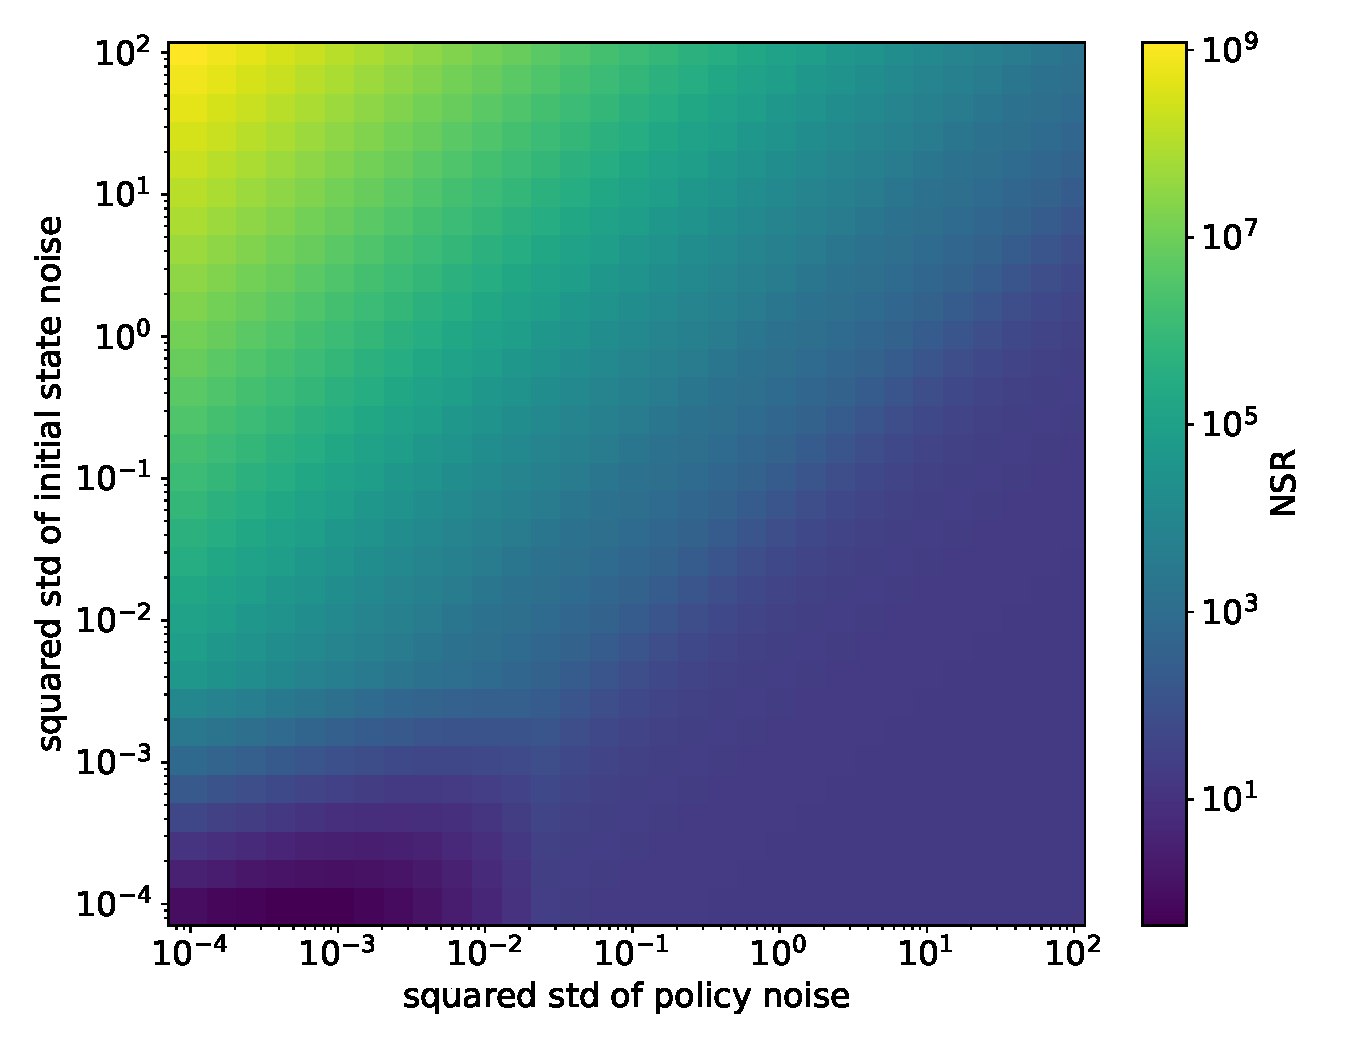
\includegraphics[width=0.4\textwidth]{figure/total_ratio_map_sigma_sigma0_lqg.pdf}
    \caption{NSR of the REINFORCE estimator in one-step LQG with isotropic \(\Sigma=\sigma^2 I\) and \(\Sigma_0=\sigma_0^2 I\) for double integrator \eqref{eq:double-integrator}.
    % From the scaling summary after Theorem~\ref{thm:lqg-variance-one-step}, NSR grows linearly with \(s_0/s\) when \(s_0\gg s\). This matches the left-up region of the heatmap where NSR is large.
    }
    \label{fig:lqr-variance-T1-scaling}
    \vspace{-4mm}
\end{figure}

% \begin{figure}
%     \centering
%     \includegraphics[width=1.0\textwidth]{figure/variance_pie_T1.pdf}
%     \caption{On random systems with random policies, term $E_{1,K}$ dominates the variance $\VarF(\hat G_K)$ for small \(\Sigma\) and large \(\Sigma_0\). Each sub-figure represents a random system-policy pair, with random \(A,B,Q_s,Q_a,K\) and varying \(\Sigma,\Sigma_0\).}
%     \label{fig:lqr-variance-E1K-dominance}
% \end{figure}

% \textbf{Effect of the feedback matrix \(K\).}
% Beyond the preceding scalings, $K$ couples with $A,B$ through $F=A+BK$. As $K$ varies, so do the eigenvalues of $F$. As $\rho(F)$ increases, the variance grows roughly quartically with $\rho(F)$.


%%%%%%%%%%%%%%%%%%%%%%%%%%%%%%%%%%%%%%%%%%%%%%%%%%%%%%%%%%%%%%%%%%%%%%%%%%%%%%%%%%%%%%%
%%% this part is for infinite-horizon variance analysis, most likely I will not use this in the final paper
%%%%%%%%%%%%%%%%%%%%%%%%%%%%%%%%%%%%%%%%%%%%%%%%%%%%%%%%%%%%%%%%%%%%%%%%%%%%%%%%%%%%%%%


% Based on the one-step variance analysis above, we turn to two estimators. The first is the classical REINFORCE policy-gradient estimator; the second is a state-visitation estimator. The REINFORCE estimator applies to both finite- and infinite-horizon objectives, whereas the state-visitation estimator is only valid in the infinite-horizon setting. In both cases, the quantities we consider are well-defined under the discounted stability condition:
% \begin{equation}\label{eq:ms-stability}
% \gamma\,\rho(F)^2<1.
% \end{equation}
% Let $\Sigma_t:=\E[s_t s_t^\top]$. From $s_{t+1}=Fs_t+B\varepsilon_t$ with $\varepsilon_t\sim\mathcal N(0,\Sigma)$,
% \[
% \Sigma_{t+1}=F\Sigma_tF^\top+W,\qquad W:=B\Sigma B^\top,
% \]
% hence
% \[
% \Sigma_t = F^t\Sigma_0(F^\top)^t+\sum_{k=0}^{t-1}F^kW(F^\top)^k.
% \]

% \begin{lemma}[Finite objective and finite REINFORCE moments under stability]
% \label{lem:reinforce-finite}
% Consider the linear-Gaussian system
% \[
% s_{t+1}=As_t+Ba_t,~ a_t=Ks_t+\varepsilon_t,~ \varepsilon_t\sim\mathcal N(0,\Sigma)\ \text{i.i.d.},
% \]
% with $s_0\sim\mathcal N(0,\Sigma_0)$ independent of $\{\varepsilon_t\}_{t\ge0}$, and define $F:=A+BK$.
% Let the stage reward be
% \[
% r_t=-\big(s_{t+1}^\top Q_s s_{t+1}+a_t^\top Q_a a_t\big),
% \qquad Q_s\succeq0,\ Q_a\succeq0,
% \]
% and fix a discount factor $0<\gamma<1$.
% Assume $\Sigma\succ0$ and $\rho(F)<1$.
% Define the infinite-horizon objective $J:=\E\big[\sum_{t=0}^\infty \gamma^t r_t\big]$ and the REINFORCE estimator
% \[
% \widehat g_K:=\sum_{t=0}^{\infty}\gamma^t\,G_t\,\nabla_K\log\pi(a_t\mid s_t),
% \qquad
% G_t:=\sum_{k=t}^{\infty}\gamma^{k-t}r_k,
% \]
% where for the Gaussian policy $\pi(\cdot\mid s_t)=\mathcal N(Ks_t,\Sigma)$,
% \[
% \nabla_K\log\pi(a_t\mid s_t)=\Sigma^{-1}\varepsilon_t s_t^\top.
% \]
% Then:
% \begin{enumerate}
% \item $|J|<\infty$.
% \item $\E\|\widehat g_K\|_{\mathrm F}<\infty$ (the estimator is integrable).
% \item $\E\|\widehat g_K\|_{\mathrm F}^2<\infty$, hence $\VarF(\widehat g_K)<\infty$.
% \end{enumerate}
% \end{lemma}

% \begin{proof}
% \textbf{Step 1: Uniform moment bounds for $s_t$ and $a_t$.}
% Write the closed-loop dynamics as
% \[
% s_{t+1}=Fs_t+B\varepsilon_t.
% \]
% Let $\Sigma_t:=\E[s_t s_t^\top]$. Then
% \begin{equation}\label{eq:Sigma-rec}
% \Sigma_{t+1}=F\Sigma_tF^\top+W,\qquad W:=B\Sigma B^\top,
% \end{equation}
% and iterating gives
% \begin{equation}\label{eq:Sigma-iter}
% \Sigma_t = F^t\Sigma_0(F^\top)^t+\sum_{k=0}^{t-1}F^kW(F^\top)^k.
% \end{equation}
% Since $\rho(F)<1$, there exist constants $C_F>0$ and $0<\beta<1$ such that
% \begin{equation}\label{eq:F-power}
% \|F^t\|_2\le C_F\,\beta^t,\qquad \forall t\ge0.
% \end{equation}
% Using~\eqref{eq:Sigma-iter} and $\tr(UXU^\top)\le \|U\|_2^2\,\tr(X)$ for $X\succeq0$, we obtain
% \[
% \tr(\Sigma_t)
% \le \|F^t\|_2^2\tr(\Sigma_0)+\sum_{k=0}^{t-1}\|F^k\|_2^2\tr(W)
% \le C_F^2\beta^{2t}\tr(\Sigma_0)+C_F^2\tr(W)\sum_{k=0}^{\infty}\beta^{2k}.
% \]
% Hence $\sup_t \E\|s_t\|_2^2=\sup_t\tr(\Sigma_t)\le C_s<\infty$ for some constant $C_s$.

% Because each $s_t$ is Gaussian and mean-zero, its fourth moment satisfies
% \[
% \E\|s_t\|_2^4
% =2\,\tr(\Sigma_t^2)+\tr(\Sigma_t)^2
% \le 3\,\tr(\Sigma_t)^2
% \le 3C_s^2,
% \]
% so $\sup_t \E\|s_t\|_2^4<\infty$. Similarly, $a_t=Ks_t+\varepsilon_t$ is Gaussian mean-zero and
% \[
% \E\|a_t\|_2^2 \le 2\|K\|_2^2\E\|s_t\|_2^2 + 2\E\|\varepsilon_t\|_2^2
% \le 2\|K\|_2^2 C_s +2\tr(\Sigma)=:C_a,
% \]
% and by the same Gaussian-moment identity, $\sup_t \E\|a_t\|_2^4<\infty$.

% \medskip
% \textbf{Step 2: The objective is finite.}
% Using $x^\top Q x\le \|Q\|_2\|x\|_2^2$,
% \[
% |r_t|
% \le \|Q_s\|_2\,\|s_{t+1}\|_2^2 + \|Q_a\|_2\,\|a_t\|_2^2.
% \]
% Taking expectations and using the uniform second-moment bounds from Step 1 yields
% $\sup_t \E|r_t|\le C_r<\infty$. Therefore,
% \[
% |J|
% \le \sum_{t=0}^{\infty}\gamma^t\,\E|r_t|
% \le \frac{C_r}{1-\gamma}
% <\infty.
% \]

% \medskip
% \textbf{Step 3: Uniform bounds for $G_t$ moments.}
% Since $G_t=\sum_{j=0}^\infty \gamma^j r_{t+j}$ and $\gamma^j\ge0$,
% \[
% \E|G_t|
% \le \sum_{j=0}^{\infty}\gamma^j\,\E|r_{t+j}|
% \le \frac{C_r}{1-\gamma}
% =:C_G.
% \]
% For the second moment, use the inequality
% \[
% \Big(\sum_{j=0}^{\infty}\gamma^j x_j\Big)^2
% \le \Big(\sum_{j=0}^{\infty}\gamma^j\Big)\Big(\sum_{j=0}^{\infty}\gamma^j x_j^2\Big)
% \quad(\gamma^j\ge0),
% \]
% with $x_j:=|r_{t+j}|$. Taking expectations gives
% \[
% \E[G_t^2]
% \le \frac{1}{1-\gamma}\sum_{j=0}^{\infty}\gamma^j\,\E[r_{t+j}^2].
% \]
% Moreover,
% \[
% r_t^2
% \le 2\|Q_s\|_2^2\|s_{t+1}\|_2^4 + 2\|Q_a\|_2^2\|a_t\|_2^4,
% \]
% so Step 1 implies $\sup_t \E[r_t^2]\le C_{r,2}<\infty$, and hence
% \begin{equation}\label{eq:G2bound}
% \sup_t \E[G_t^2]\le \frac{C_{r,2}}{(1-\gamma)^2}=:C_{G,2}<\infty.
% \end{equation}

% \medskip
% \textbf{Step 4: Integrability of the REINFORCE estimator.}
% Write
% \[
% \nabla_K\log\pi(a_t\mid s_t)=\Sigma^{-1}\varepsilon_t s_t^\top,
% \qquad
% \|\Sigma^{-1}\varepsilon_t s_t^\top\|_{\mathrm F}
% =\|\Sigma^{-1}\varepsilon_t\|_2\,\|s_t\|_2.
% \]
% Because $s_t$ depends only on $\varepsilon_0,\dots,\varepsilon_{t-1}$, it is independent of $\varepsilon_t$,
% so by Cauchy--Schwarz,
% \[
% \E\|\Sigma^{-1}\varepsilon_t s_t^\top\|_{\mathrm F}
% \le \sqrt{\E\|\Sigma^{-1}\varepsilon_t\|_2^2}\,\sqrt{\E\|s_t\|_2^2}
% \le \sqrt{\tr(\Sigma^{-1})}\,\sqrt{C_s}
% =:C_\nabla.
% \]
% Also, by Cauchy--Schwarz and~\eqref{eq:G2bound},
% \[
% \E\big[|G_t|\,\|\nabla_K\log\pi(a_t\mid s_t)\|_{\mathrm F}\big]
% \le \sqrt{\E[G_t^2]}\,\sqrt{\E\|\nabla_K\log\pi(a_t\mid s_t)\|_{\mathrm F}^2}
% \le \sqrt{C_{G,2}}\,\sqrt{\tr(\Sigma^{-1})\,C_s}
% =:C_1.
% \]
% Therefore,
% \[
% \E\|\widehat g_K\|_{\mathrm F}
% \le \sum_{t=0}^{\infty}\gamma^t\,\E\big[|G_t|\,\|\nabla_K\log\pi(a_t\mid s_t)\|_{\mathrm F}\big]
% \le \sum_{t=0}^{\infty}\gamma^t\,C_1
% =\frac{C_1}{1-\gamma}
% <\infty,
% \]
% proving integrability.

% \medskip
% \textbf{Step 5: Finite variance.}
% Using $\| \sum_t X_t\|_{\mathrm F}\le \sum_t \|X_t\|_{\mathrm F}$ and the weighted Cauchy--Schwarz inequality,
% \[
% \Big(\sum_{t=0}^\infty \gamma^t u_t\Big)^2
% =\Big(\sum_{t=0}^\infty \sqrt{\gamma^t}\cdot \sqrt{\gamma^t}u_t\Big)^2
% \le \Big(\sum_{t=0}^\infty \gamma^t\Big)\Big(\sum_{t=0}^\infty \gamma^t u_t^2\Big),
% \]
% with $u_t:=|G_t|\,\|\nabla_K\log\pi(a_t\mid s_t)\|_{\mathrm F}$, we get
% \[
% \|\widehat g_K\|_{\mathrm F}^2
% \le \frac{1}{1-\gamma}\sum_{t=0}^{\infty}\gamma^t\,G_t^2\,\|\nabla_K\log\pi(a_t\mid s_t)\|_{\mathrm F}^2.
% \]
% Taking expectations and applying Cauchy--Schwarz,
% \[
% \E\big[G_t^2\,\|\nabla_K\log\pi(a_t\mid s_t)\|_{\mathrm F}^2\big]
% \le \sqrt{\E[G_t^4]}\,\sqrt{\E\|\nabla_K\log\pi(a_t\mid s_t)\|_{\mathrm F}^4}.
% \]
% Since $(s_t,a_t)$ are Gaussian with uniformly bounded covariance (Step 1), all polynomial moments of $r_t$
% are uniformly bounded, which implies $\sup_t \E[G_t^4]<\infty$ by the same geometric-weight argument used for~\eqref{eq:G2bound}.
% Also, independence of $(\varepsilon_t,s_t)$ gives
% \[
% \E\|\nabla_K\log\pi(a_t\mid s_t)\|_{\mathrm F}^4
% =\E\|\Sigma^{-1}\varepsilon_t\|_2^4\ \E\|s_t\|_2^4
% <\infty
% \quad\text{and is uniformly bounded in $t$}.
% \]
% Therefore there exists a constant $C_2<\infty$ such that
% $\sup_t \E[G_t^2\|\nabla_K\log\pi(a_t\mid s_t)\|_{\mathrm F}^2]\le C_2$, and hence
% \[
% \E\|\widehat g_K\|_{\mathrm F}^2
% \le \frac{1}{1-\gamma}\sum_{t=0}^{\infty}\gamma^t\,C_2
% =\frac{C_2}{(1-\gamma)^2}
% <\infty.
% \]
% Finally, $\VarF(\widehat g_K)=\E\|\widehat g_K\|_{\mathrm F}^2-\|\E[\widehat g_K]\|_{\mathrm F}^2<\infty$.
% \end{proof}

\subsection{NSR of the Multi-step REINFORCE Estimator}\label{sec:multi-step-lqg}

We reduce the \(T\)-step system to a larger one-step system by lifting the dynamics and the policy to block form.

\begin{theorem}[Lifted \(T\)-step system]\label{thm:lqr-lift}
Let the stacked states, actions, and noises be
  \begin{align*}
      \bar s :=\begin{bmatrix}s_0\\ \vdots\\ s_{T-1}\end{bmatrix}\in\mathbb R^{nT},\quad
      \bar s^+:=\begin{bmatrix}s_1\\ \vdots\\ s_T\end{bmatrix}\in\mathbb R^{nT},\quad \\
      \bar a:=\begin{bmatrix}a_0\\ \vdots\\ a_{T-1}\end{bmatrix}\in\mathbb R^{mT},\quad
      \bar \varepsilon:=\begin{bmatrix}\varepsilon_0\\ \vdots\\ \varepsilon_{T-1}\end{bmatrix}\in\mathbb R^{mT}.
  \end{align*}
There exist matrices
  \begin{align*}
  \mathcal F_S,\ \mathcal F_S^+ \in \mathbb R^{nT\times n},\quad \mathcal F_E, \ \mathcal F_E^+ \in \mathbb R^{nT\times mT}\\
  \mathcal K_S\in\mathbb R^{mT\times n},\ \ \mathcal K_E\in\mathbb R^{mT\times mT},
  \end{align*}
  such that
  \[
  \bar s=\mathcal F_S s_0+\mathcal F_E \bar\varepsilon,\ \ 
  \bar s^+=\mathcal F_S^+ s_0+\mathcal F_E^+ \bar\varepsilon,\ \ 
  \bar a=\mathcal K_S s_0+\mathcal K_E \bar\varepsilon.
  \]
Let \(D_\gamma:=\mathrm{diag}(\gamma^0,\gamma^1,\ldots,\gamma^{T-1})\) and define the discounted block weights
\[
\mathsf Q_{s,\gamma}:=D_\gamma\otimes Q_s,\quad
\mathsf Q_{a,\gamma}:=D_\gamma\otimes Q_a,\quad
\overline\Sigma:=I_T\otimes \Sigma.
\]
Then the discounted return admits a single-step quadratic decomposition
\begin{align}\label{eq:lqr-lift-discount-decompose}
&R(\tau)=-(x+2y+z), \\
&x:=s_0^\top \overline M_{ss} s_0,\;\;
y:=s_0^\top \overline M_{se}\,\bar \varepsilon,\;\;
z:=\bar \varepsilon^\top \overline M_{ee}\,\bar \varepsilon,
\end{align}
where the lifted blocks are
\begin{align}
\overline M_{ss}&:= {\mathcal F_S^+}^\top \mathsf Q_{s,\gamma} \mathcal F_S^+ +\mathcal K_S^\top \mathsf Q_{a,\gamma} \mathcal K_S, \label{eq:lqr-lift-discount-Mss}\\
\overline M_{se}&:= {\mathcal F_S^+}^\top \mathsf Q_{s,\gamma} \mathcal F_E^+ +\mathcal K_S^\top \mathsf Q_{a,\gamma} \mathcal K_E, \label{eq:lqr-lift-discount-Mse}\\
\widebar M_{ee}&:= {\mathcal F_E^+}^\top \mathsf Q_{s,\gamma} \mathcal F_E^+ +\mathcal K_E^\top \mathsf Q_{a,\gamma} \mathcal K_E. \label{eq:lqr-lift-discount-Mee}
\end{align}
\end{theorem}
With the lifted one-step system, we can study the variance and gradients of the REINFORCE estimator.
% To study the variance of \(\widehat G_K\), expand it as $T^2$ terms and use python to calculate the fourth-order moments of Gaussian variables. 
% $$
% \E[\|\widehat G_K\|_{\mathrm{F}}^2] = \E [(\Big(\sum_{t=0}^{T-1} \xi_t\,s_t^\top\Big)^\top\Big(\sum_{t=0}^{T-1} \xi_t\,s_t^\top\Big)\,R(\tau)^2)]
% $$

% expand it as $T^2$ terms:
% $$
% \E[\|\widehat G_K\|_{\mathrm{F}}^2] = \sum_{t=0}^{T-1}\sum_{p=0}^{T-1} \E [ (\xi_t^\top \xi_p) (s_t^\top s_p) R(\tau)^2 ]
% $$

\begin{theorem}[Variance and gradients of multi-step LQG]
\label{thm:lqr-variance-T-compose}
Consider the lifted multi-step LQG in Theorem~\ref{thm:lqr-lift}, the following statements hold.

\textbf{(i) Second moments.}
With the lifted notation $R(\tau)=-(x+2y+z)$ and the shorthand
$\mathrm{IS}_\Omega(\cdot)$ of Lemma~\ref{lem:IS_shorthand}, we have the decompositions of the second moments:
$$
\mathbb E\!\left[\|\widehat G_K\|_{\mathrm F}^2\right]=\!\!\!\sum_{t,p=0}^{T-1}\sum_{i=1}^{6}E^{K}_{i,tp},\ \ 
\mathbb E\!\left[\|\widehat G_\ell\|_{2}^2\right]=\!\!\!\sum_{t,p=0}^{T-1}\sum_{i=1}^{4}E^{\ell}_{i,tp}
$$
where the terms $E^{K}_{1,tp},\dots,E^{K}_{6,tp}$ are given by the six-term decompositions \eqref{eq:EtpFtp_def}--\eqref{eq:Ftp_final} in the proof, and $E^{\ell}_{1,tp},\dots,E^{\ell}_{4,tp}$ are given by
\eqref{eq:Atp_ell_final}, \eqref{eq:Btp_ell_final}, \eqref{eq:Ctp_ell_final}, \eqref{eq:Dtp_ell_final}.

\textbf{(ii) Mean gradients.}
Let $P_t:=\mathrm{Cov}(s_t)$ satisfy the covariance recursion
\[
P_{t+1}=F P_t F^\top + B\Sigma B^\top,\quad P_0=\Sigma_0
\]
and let $\{\Lambda_t\}_{t=1}^{T}$ satisfy the backward recursion
\[
\Lambda_T=\tfrac{1}{\gamma}Q_s,\quad
\Lambda_t=\tfrac{1}{\gamma}Q_s + K^\top Q_a K + \gamma F^\top \Lambda_{t+1} F.
\]
Then the gradients of the objective $J(K,\Sigma)$ are
\begin{align}
\nabla_K J
&=
-2\sum_{t=0}^{T-1}\gamma^{t}\Big( Q_a K P_t \;+\; \gamma\, B^\top \Lambda_{t+1} F\, P_t \Big)\label{eq:mean_grad_K},\!\!\\
\nabla_{\ell} J 
&=
-2\mathrm{diag}(\Sigma\sum_{t=0}^{T-1}\gamma^t\Big( Q_a + \gamma B^\top \Lambda_{t+1} B \Big)).
\end{align}
\end{theorem}

\begin{corollary}[Stationary points of $J(K,\Sigma)$]
\label{cor:lqg_stationary}
Under the assumptions of Theorem~\ref{thm:lqr-variance-T-compose}, if $Q_a \succ 0$, then $\nabla_\ell J=0$ if and only if $\Sigma=\mathbf 0$.
\end{corollary}

Theorem~\ref{thm:lqr-variance-T-compose} provides an exact numerical procedure for computing the REINFORCE estimator's variance (and NSR) in any finite-horizon LQG system. The resulting expressions are considerably more involved than in the one-step case, making it difficult to directly extract clean scaling laws. We therefore analyze a simple upper bound to clarify how the NSR scales with the horizon, the policy and initial-state covariances, and closed-loop stability.

%%%%%%%%%%%%%%%%%%%%%%%%%%%%%%%%%%%%%%%%%%%%%%%%%%%%%%%%%%%%%%%%%%%%%%%%%%%%%%%%%%%%%%%
%%% this box is to discuss why we cannot get a matching lower bound, but no use in paper
%%%%%%%%%%%%%%%%%%%%%%%%%%%%%%%%%%%%%%%%%%%%%%%%%%%%%%%%%%%%%%%%%%%%%%%%%%%%%%%%%%%%%%%

% \begin{takeawaybox}{Can we obtain a matching lower bound?}
%   The Cauchy--Schwarz step
%   \[
%   \mathbb E\big[\|\widehat G_K\|_{\mathrm{F}}^2\big]
%   \;\le\;
%   \mathbb E\Big[\Big(\sum_{t=0}^{T-1} \|\xi_t\|_2^2\Big)
%   \Big(\sum_{t=0}^{T-1} \|s_t\|_2^2\Big) R(\tau)^2\Big]
%   \]
%   is one–sided. This is impossible to get a lower bound because $\Big\|\sum_{t=0}^{T-1} \xi_t\,s_t^\top\Big\|_{\mathrm{F}}^2 \geq c \Big(\sum_{t=0}^{T-1} \|\xi_t\|_2^2\Big) \Big(\sum_{t=0}^{T-1} \|s_t\|_2^2\Big)$ does not hold for any $c$. Another try is to use the AM--GM/Cauchy inequality on the time index,
%   \[
%   \Big\|\sum_{t=0}^{T-1} \xi_t s_t^\top\Big\|_{\mathrm{F}}^2
%   \;\le\;
%   T \sum_{t=0}^{T-1} \|\xi_t\|_2^2 \|s_t\|_2^2,
%   \]
%   we obtain another upper bound
%   \[
%   \mathbb E\big[\|\widehat G_K\|_{\mathrm{F}}^2\big]
%   \;\le\;
%   T\,\mathbb E\Big[\sum_{t=0}^{T-1} \|\xi_t\|_2^2 \|s_t\|_2^2 R(\tau)^2\Big].
%   \]

%   A natural hope would be to use the “diagonal” terms
%   \(\|\xi_t\|_2^2 \|s_t\|_2^2 R(\tau)^2\) to derive a lower bound. However, when we expand
%   \(\big\|\sum_t \xi_t s_t^\top\big\|_{\mathrm{F}}^2 R(\tau)^2\), the cross terms
%   \(\xi_t \xi_p^\top s_t s_p^\top R(\tau)^2\) (with \(t\neq p\)) involve mixed fourth- and sixth-order Gaussian moments. Even though \(R(\tau)\) is quadratic in \((s_0,\bar\varepsilon)\) and each \(s_t\) is linear, Wick’s formula shows that these cross terms do not vanish and are not sign–definite in general. \red{Need to check carefully if there is counter example.}

%   You will see later in the generic nonlinear case that although we don't know what is the cross term, we can show the diagonal part scale with $\tr(\Sigma^{-1})$ but the off-diagonal doesn't, so the off-diagonal will vanish compare to the diagonal part when $\Sigma$ is small. Thus we can say
%   \[
%   \mathbb E\big[\|\widehat G_K\|_{\mathrm{F}}^2\big]
%   \approx
%   \,\mathbb E\Big[\sum_{t=0}^{T-1} \|\xi_t\|_2^2 \|s_t\|_2^2 R(\tau)^2\Big].
%   \]
%   is a good approximation when $\Sigma$ is small. \red{But for the right hand side we don't have a clean close form, if we expand it similar to Theorem~\ref{thm:lqg-variance-one-step} we will have a sum over time which is hard to analysis.}
% \end{takeawaybox}


\begin{figure*}[h]
    \centering
    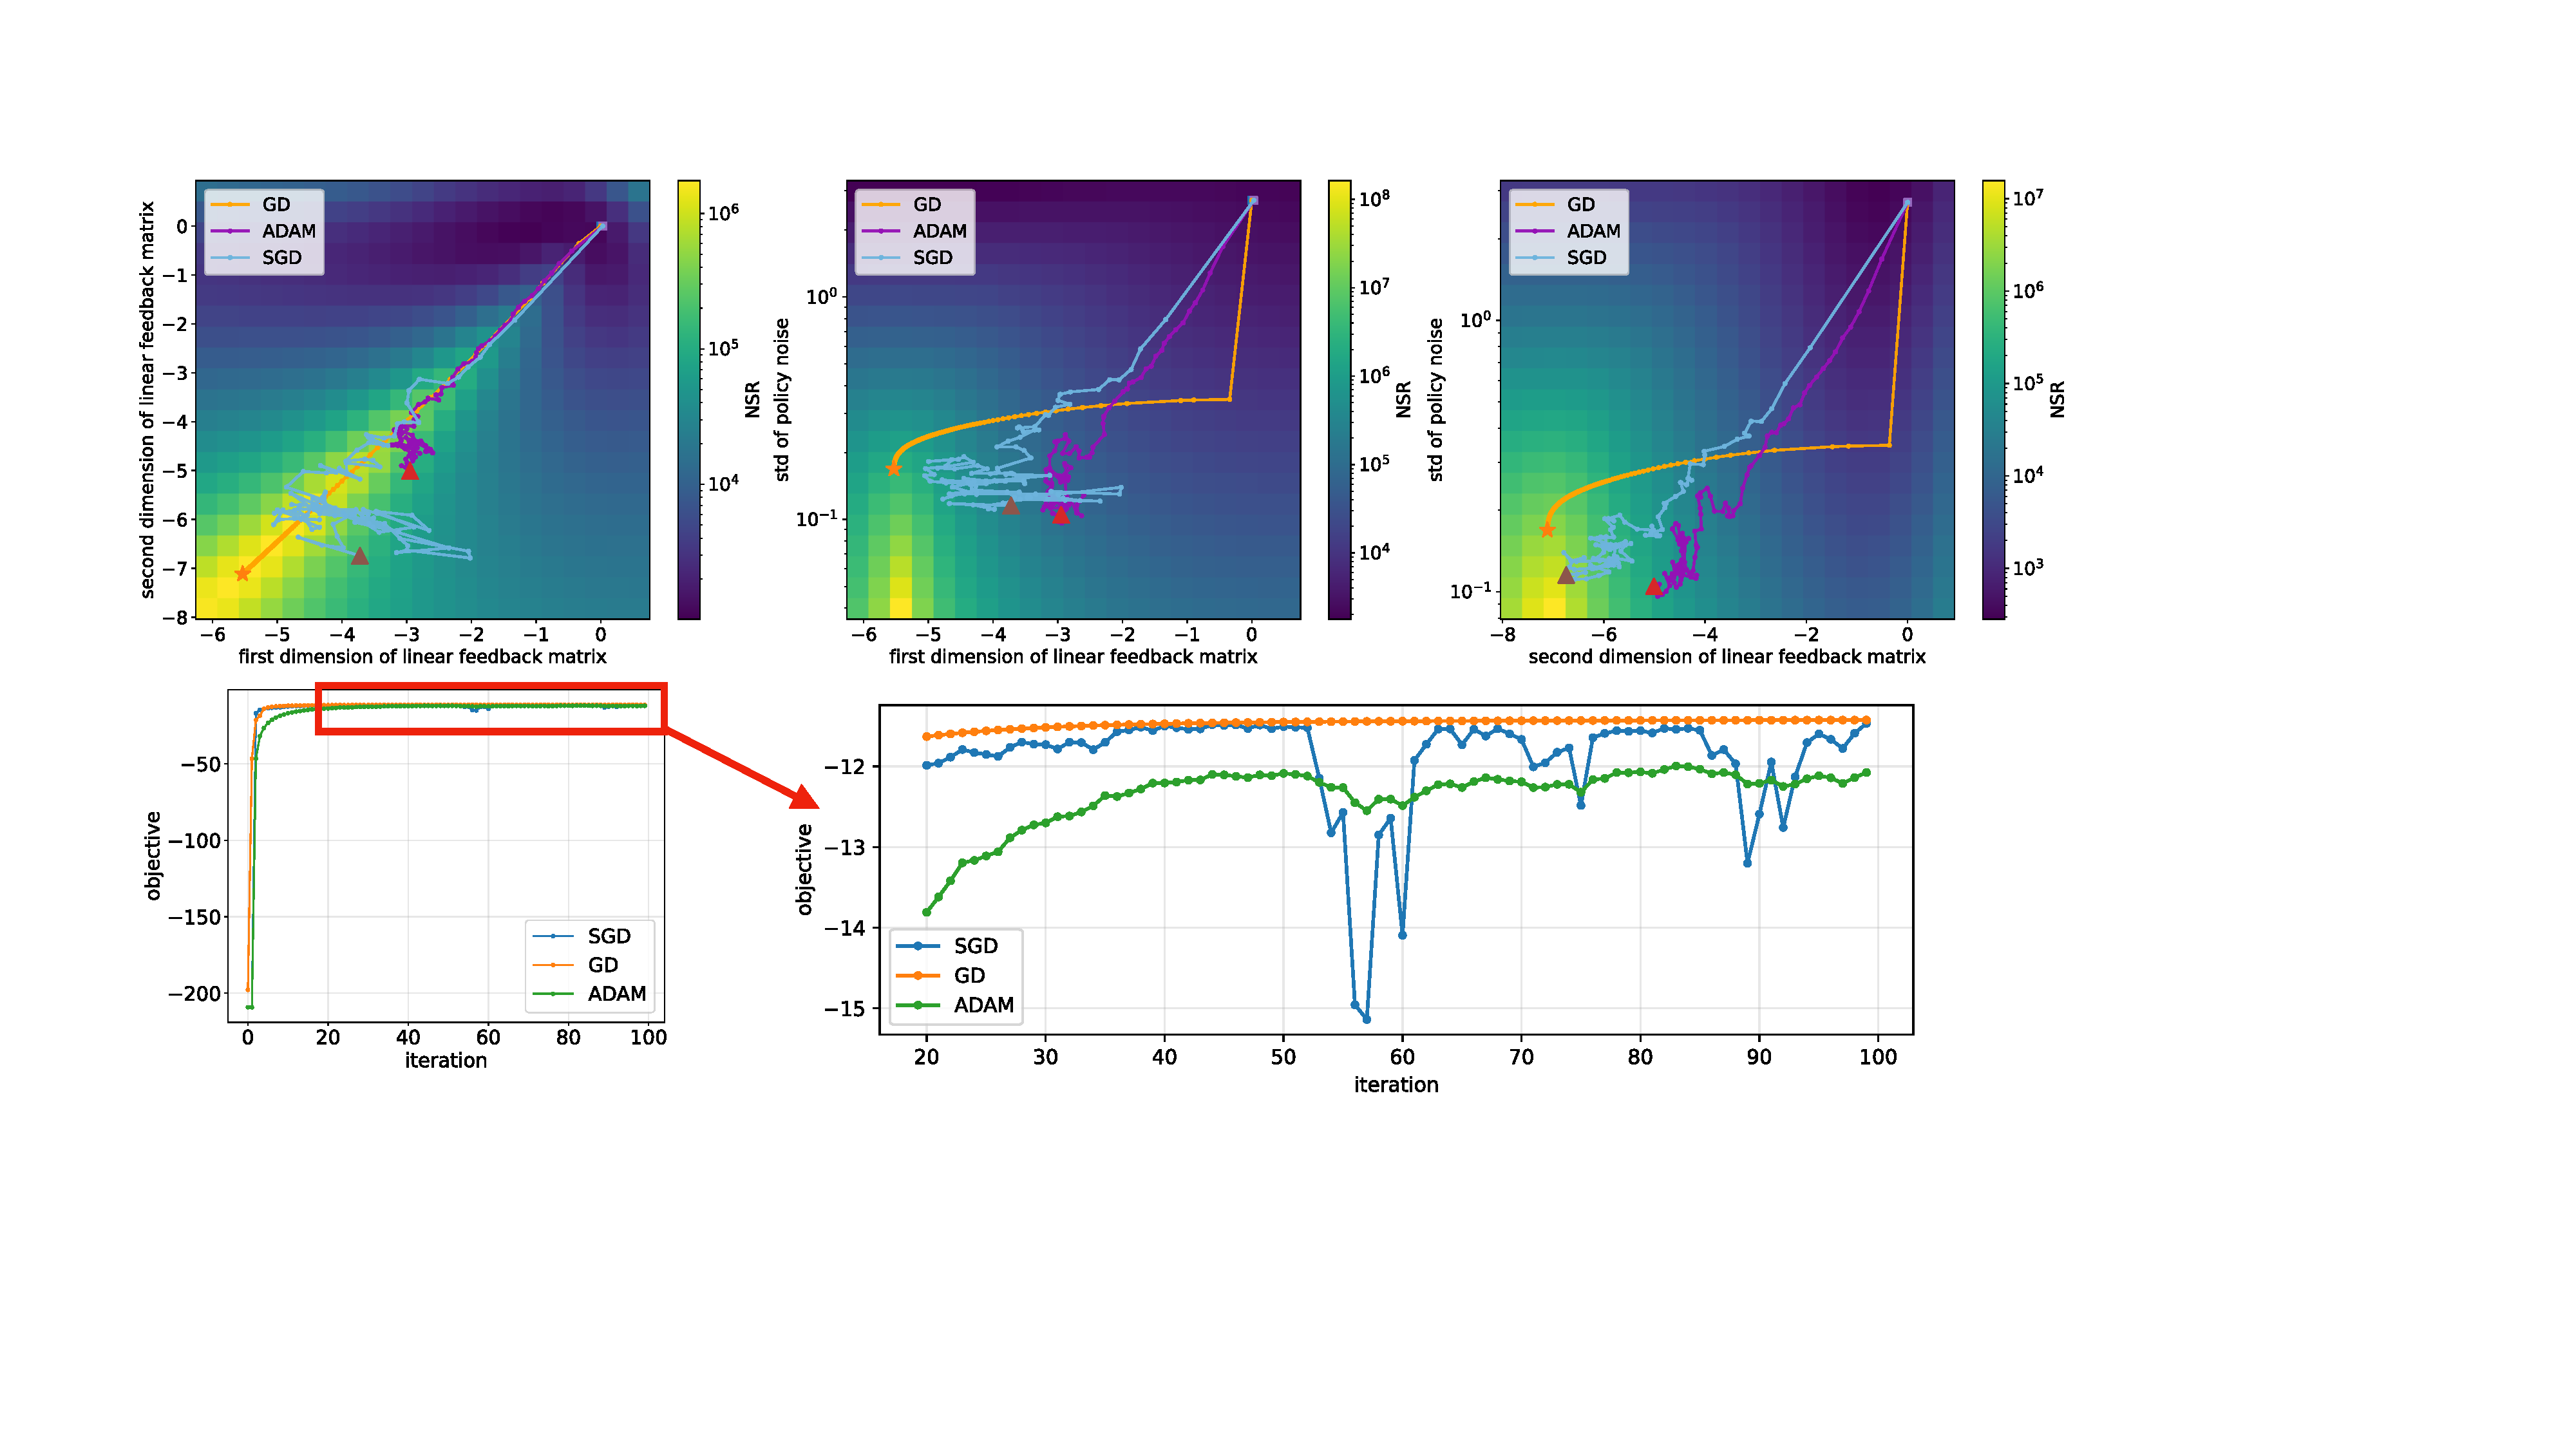
\includegraphics[width=0.86\textwidth]{figure/ratio_map_linear.pdf}
    \caption{NSR and objective along optimization trajectories on a double-integrator system with $T=30$. {Top}: optimizer trajectories overlaid on the NSR landscape. {Bottom}: learning curves (objective vs.\ iteration). The three optimizers (GD, SGD, Adam) start from the same initial policy (square), move toward the optimal policy (star), and terminate at triangles. The NSR increases markedly as the policy approaches optimality, consistent with our theory. As the NSR grows, SGD and Adam exhibit oscillations in the learning curves.}
    \label{fig:lqr-variance-traj}
    \vspace{-4mm}
\end{figure*}

\begin{theorem}[Multi-step LQG variance bound]\label{thm:lqr-variance-T-bound}
Under the lifted multi-step LQG in Theorem~\ref{thm:lqr-lift}, we have
\begin{align}\label{eq:K-variance-split-clean}
  \VarF(\widehat G_K)
  &\;\le\;2\underbrace{\mathbb E\big[\|\overline\Sigma^{-1}\bar\varepsilon\|_2^2\,
                              \|\mathcal F_S s_0\|_2^2\,R(\tau)^{2}\big]}_{(\star)} \nonumber \\
  &\;+\;2\underbrace{\mathbb E\big[\|\overline\Sigma^{-1}\bar\varepsilon\|_2^2\,
                              \|\mathcal F_E\bar\varepsilon\|_2^2\,R(\tau)^{2}\big]}_{(\dagger)},
\end{align}
\vspace{-3mm}
\begin{equation}\label{eq:ell-second-moment-bound}
\VarF(\widehat G_\ell) 
\;\le\;
T\,\mathbb E\big[(2\|\overline\Sigma^{-1/2}\bar\varepsilon\|_2^4+2mT)\,R(\tau)^2\big],
\end{equation}
and the expectation on the right-hand side admits an explicit Gaussian-moment expansion given in \eqref{eq:star-final}, \eqref{eq:dagger-final} and \eqref{eq:Ell-final}.
\end{theorem}

\textbf{Analysis of NSR.} Same as the analysis in the one-step case, $\overline M_{ee}, \overline M_{ss} \succeq 0, \overline M_{se}$ are nonzero matrices, so that every term in $(\star)$, $(\dagger)$ and $\E\!\left[\|\widehat G_\ell\|_2^2\right]$ are nonzero. With $\Sigma = \sigma^2 I$ and $\Sigma_0 = \sigma_0^2 I$, we can write these terms as
\begin{align*}
\vspace{-2mm}
&(\star) = \Theta(\frac{\sigma_0^6}{\sigma^2} + \sigma_0^4 + \sigma_0^2 \sigma^2), \quad (\dagger) = \Theta(\sigma^4 + \sigma_0^4 + \sigma_0^2 \sigma^2),\\
& \E\!\left[\|\widehat G_\ell\|_2^2\right] = \Theta(\sigma^4 + \sigma_0^4 + \sigma_0^2 \sigma^2).
\vspace{-2mm}
\end{align*}
From Theorem~\ref{thm:lqr-variance-T-compose} we know $\|\mathbb{E}[\widehat G_K]\|_{\mathrm{F}}^2, \|\mathbb{E}[\widehat G_\ell]\|_2^2= \Theta((\sigma^2 + \sigma_0^2)^2)$ if they are nonzero, thus
$$
\frac{\VarF(\widehat G_K)\!+\!\VarF(\widehat G_\ell)}{\|\mathbb{E}[\widehat G_K]\|_{\mathrm{F}}^2 + \|\mathbb{E}[\widehat G_\ell]\|_{\mathrm{F}}^2}\!=O\left(\frac{\frac{\sigma_0^6}{\sigma^2} +\!\sigma_0^4 +\!\sigma_0^2 \sigma^2 +\!\sigma^4}{(\sigma_0^2 + \sigma^2)^2}\right).
$$
Again, define $\alpha:=\sigma_0^2/\sigma^2$, we have
\[
\frac{\frac{\sigma_0^6}{\sigma^2}+\sigma_0^4+\sigma_0^2 \sigma^2+\sigma^4}{(\sigma_0^2+\sigma^2)^2}
=\frac{\sigma_0^4+\sigma^4}{\sigma^2(\sigma_0^2+\sigma^2)}
=\frac{\alpha^2+1}{\alpha+1}.
\]
Therefore, if $\sigma_0 \gg \sigma$, we have \(\alpha \to \infty\) and the ratio scales as \(O(\tr(\Sigma_0)\tr(\Sigma^{-1}))\), same as in the one-step case but stated here as an upper bound.

% The verification code can be found in \texttt{Gradient/verify_multistep.py}. Easy to see these terms share the same scaling patterns as in the one-step case, but with lifted blocks. We see that $(\star)$ and $(\dagger)$ grow with \(\Sigma,\Sigma_0,K\) as before. A key additional factor is the $T$-dependence of \(\|\mathcal F_S\|_2,\|\mathcal F_E\|_2,\|\overline M_{ss}\|_2,\|\overline M_{se}\|_2,\|\overline M_{ee}\|_2\). To verify the bound, we show the pie chart and the tightness of the bound.

% \begin{table}[H]\label{tab:lqg-variance-T}
%   \centering
%   \begin{tabular}{cccc}
%   \hline
%   $\operatorname{Var}_F(G)$
%   & $\|\mathbb{E}[G]\|_{\mathrm{F}}^2$
%   & $\dfrac{\operatorname{Var}_F(G)}{\|\mathbb{E}[G]\|_{\mathrm{F}}^2}$
%   & Bound \\
%   \hline
%   $7.043467 \times 10^{8}$  & $5.229593 \times 10^{1}$  & $1.347 \times 10^{7}$ & $1.408554 \times 10^{10}$ \\
%   $7.082831 \times 10^{2}$  & $6.365420 \times 10^{-3}$ & $1.113 \times 10^{5}$ & $1.414268 \times 10^{4}$  \\
%   $2.734101 \times 10^{5}$  & $9.273833 \times 10^{1}$  & $2.948 \times 10^{3}$ & $5.321196 \times 10^{6}$  \\
%   $2.239468 \times 10^{2}$  & $3.683913$                & $6.079 \times 10^{1}$ & $3.982091 \times 10^{3}$  \\
%   \hline
%   \end{tabular}
%   \caption{Summary of variance, mean-squared norm, ratio, and new RHS bound.}
% \end{table}

% From Table~\ref{tab:lqg-variance-T} we see the ratio follows the same pattern as before. From Theorem~\ref{thm:lqg-variance-T} we know that $A,B,C,D$ terms all scale with \(\Sigma,\Sigma_0,K\) as before, but the gradient now has complex dependence on $\Sigma$ and $\Sigma_0$, but approximately $\|\mathbb{E}[G]\|_{\mathrm{F}}^2 \approx O(\Sigma^2 + \Sigma_0^2)$, thus the ratio still grows roughly linearly with \(\tr(\Sigma^{-1})\) and \(\tr(\Sigma_0)\) when \(\Sigma\) is small and \(\Sigma_0\) is large. We also show the pie chart Figure~\ref{fig:lqr-variance-AK-dominance-T} that the $A^\star$ term still dominate.

% \begin{figure}
%   \centering
%   \includegraphics[width=1.0\textwidth]{figure/variance_pie_T.pdf}
%   \caption{On random systems with random policies. It shows the same trend as Figure~\ref{fig:lqr-variance-E1K-dominance}.}
%   \label{fig:lqr-variance-AK-dominance-T}
% \end{figure}

% To assess the tightness of the bound, we report four random policies in Table~\ref{tab:lqg-variance-T-tightness}. We fix the horizon to $T=10$, the initial-state covariance to $\Sigma_0 = I_2$, and draw the noise covariance $\Sigma$ from a Gaussian ensemble. For all four policies, the ratio $\mathbb{E}[\|G\|_{\mathrm{F}}^2]/\text{(new RHS)}$ is around $0.05$. This is consistent with our derivation: the Cauchy--Schwarz inequality step can introduce a factor on the order of $T$, and the separation of the contributions of $s_0$ and $\bar\varepsilon$ may introduce an additional factor of~$2$.

% \begin{table}[h]\label{tab:lqg-variance-T-tightness}
%   \centering
%   \begin{tabular}{ccc}
%   \hline
%   $\mathbb{E}[\|G\|_{\mathrm{F}}^2]$
%   & New RHS via $2((*)+(\dagger))$
%   & Ratio $\mathbb{E}[\|G\|_{\mathrm{F}}^2]$/new RHS \\
%   \hline
%   $4.076647 \times 10^{3}$   & $7.484605 \times 10^{4}$   & $0.054$ \\
%   $1.308150 \times 10^{15}$  & $3.277439 \times 10^{16}$  & $0.040$ \\
%   $1.547068 \times 10^{5}$   & $3.011068 \times 10^{6}$   & $0.051$ \\
%   $1.727503 \times 10^{12}$  & $3.228974 \times 10^{13}$  & $0.054$ \\
%   \hline
%   \end{tabular}
%   \caption{Random system: comparison of $\mathbb{E}[\|G\|_{\mathrm{F}}^2]$, the new RHS bound, and their ratio.}
%   \end{table}

Theorem \ref{thm:lqr-variance-T-bound} further indicates the variance bound depends on the spectral norms of the lifted state maps \(\mathcal F_S\) and \(\mathcal F_E\), which exponentially grow with the horizon \(T\) if the closed-loop system is unstable. 

\begin{theorem}[Spectral norm of lifted state map]
  \label{thm:lqr-lifted-state-maps-bound}
  The lifted state map $\mathcal F_S$ satisfies
  \begin{align}
    \vspace{-2mm}
    \max_{0\le t\le T-1}\|F^t\|_2^2
    \;\le\;
    \|\mathcal F_S\|_2^2
    \;\le\;
    \sum_{t=0}^{T-1}\|F^t\|_2^2. \label{eq:FS-sandwich}
    \vspace{-2mm}
  \end{align}
  Thus, $\|\mathcal F_S\|_2^2$ is $O(1)$ if $\rho(F)<1$, and $O\big(\rho(F)^{2T}\big)$ if $\rho(F)>1$ (with \(\rho(\cdot)\) denoting the spectral radius).
\end{theorem}
Figure~\ref{fig:lqr-variance-exponential-increase} illustrates how the \emph{true} variance $\VarF(\widehat G)$ (computed exactly from Theorem~\ref{thm:lqr-variance-T-compose}) scales with the horizon $T$ across four systems: it remains bounded when $\rho(F)<1$, grows roughly polynomially when $\rho(F)=1$, and grows exponentially when $\rho(F)>1$. This verifies the prediction of Theorems~\ref{thm:lqr-variance-T-bound} and \ref{thm:lqr-lifted-state-maps-bound}.
Thus, in long-horizon tasks, closed-loop instability can dramatically worsen the NSR.

\vspace{-3mm}
\begin{figure}[h]
  \centering
  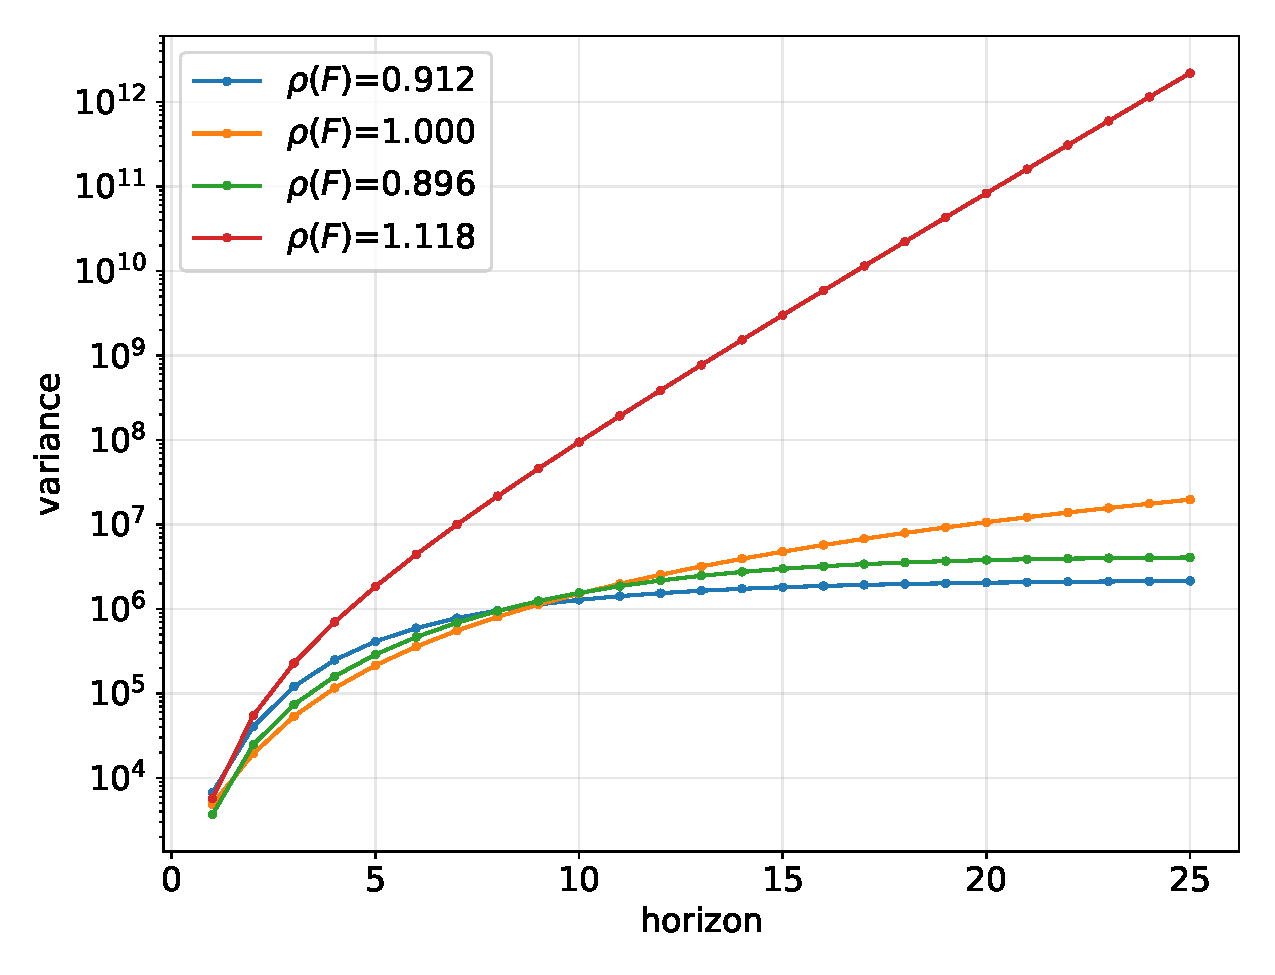
\includegraphics[width=0.82\linewidth]{figure/variance_vs_T.pdf}
  \caption{Variance growth as a function of the horizon \(T\) for four 2D systems (1D control) with varying \(\rho(F)\). We fix the initial-state covariance at \(\Sigma_0 = I_2\) and the policy covariance at \(\Sigma = 0.1 I_1\).}
  \label{fig:lqr-variance-exponential-increase}
  \vspace{-3mm}
\end{figure}

\subsection{Experiments}\label{sec:lqg-experiment}
\vspace{-1mm}

Figure~\ref{fig:lqr-variance-traj} visualizes the NSR landscape for a double-integrator system and overlays the optimization trajectories of three methods: GD, SGD, and Adam~\cite{kingma14arxiv-adam}. The policy has three parameters: a 2D gain matrix $K$ and a 1D log-std $\ell$. We observe that the NSR increases as the iterates approach the optimum. GD converges smoothly, whereas SGD and Adam exhibit oscillations once the NSR becomes large. This behavior is consistent with Corollary~\ref{cor:lqg_stationary}, which implies that the optimal policy is deterministic (\ie $\Sigma \to \mathbf 0$), so the NSR diverges near optimality; empirically, SGD and Adam are stable early on but oscillate near the optimum in both parameter space and objective value.

\begin{figure}
  \centering
  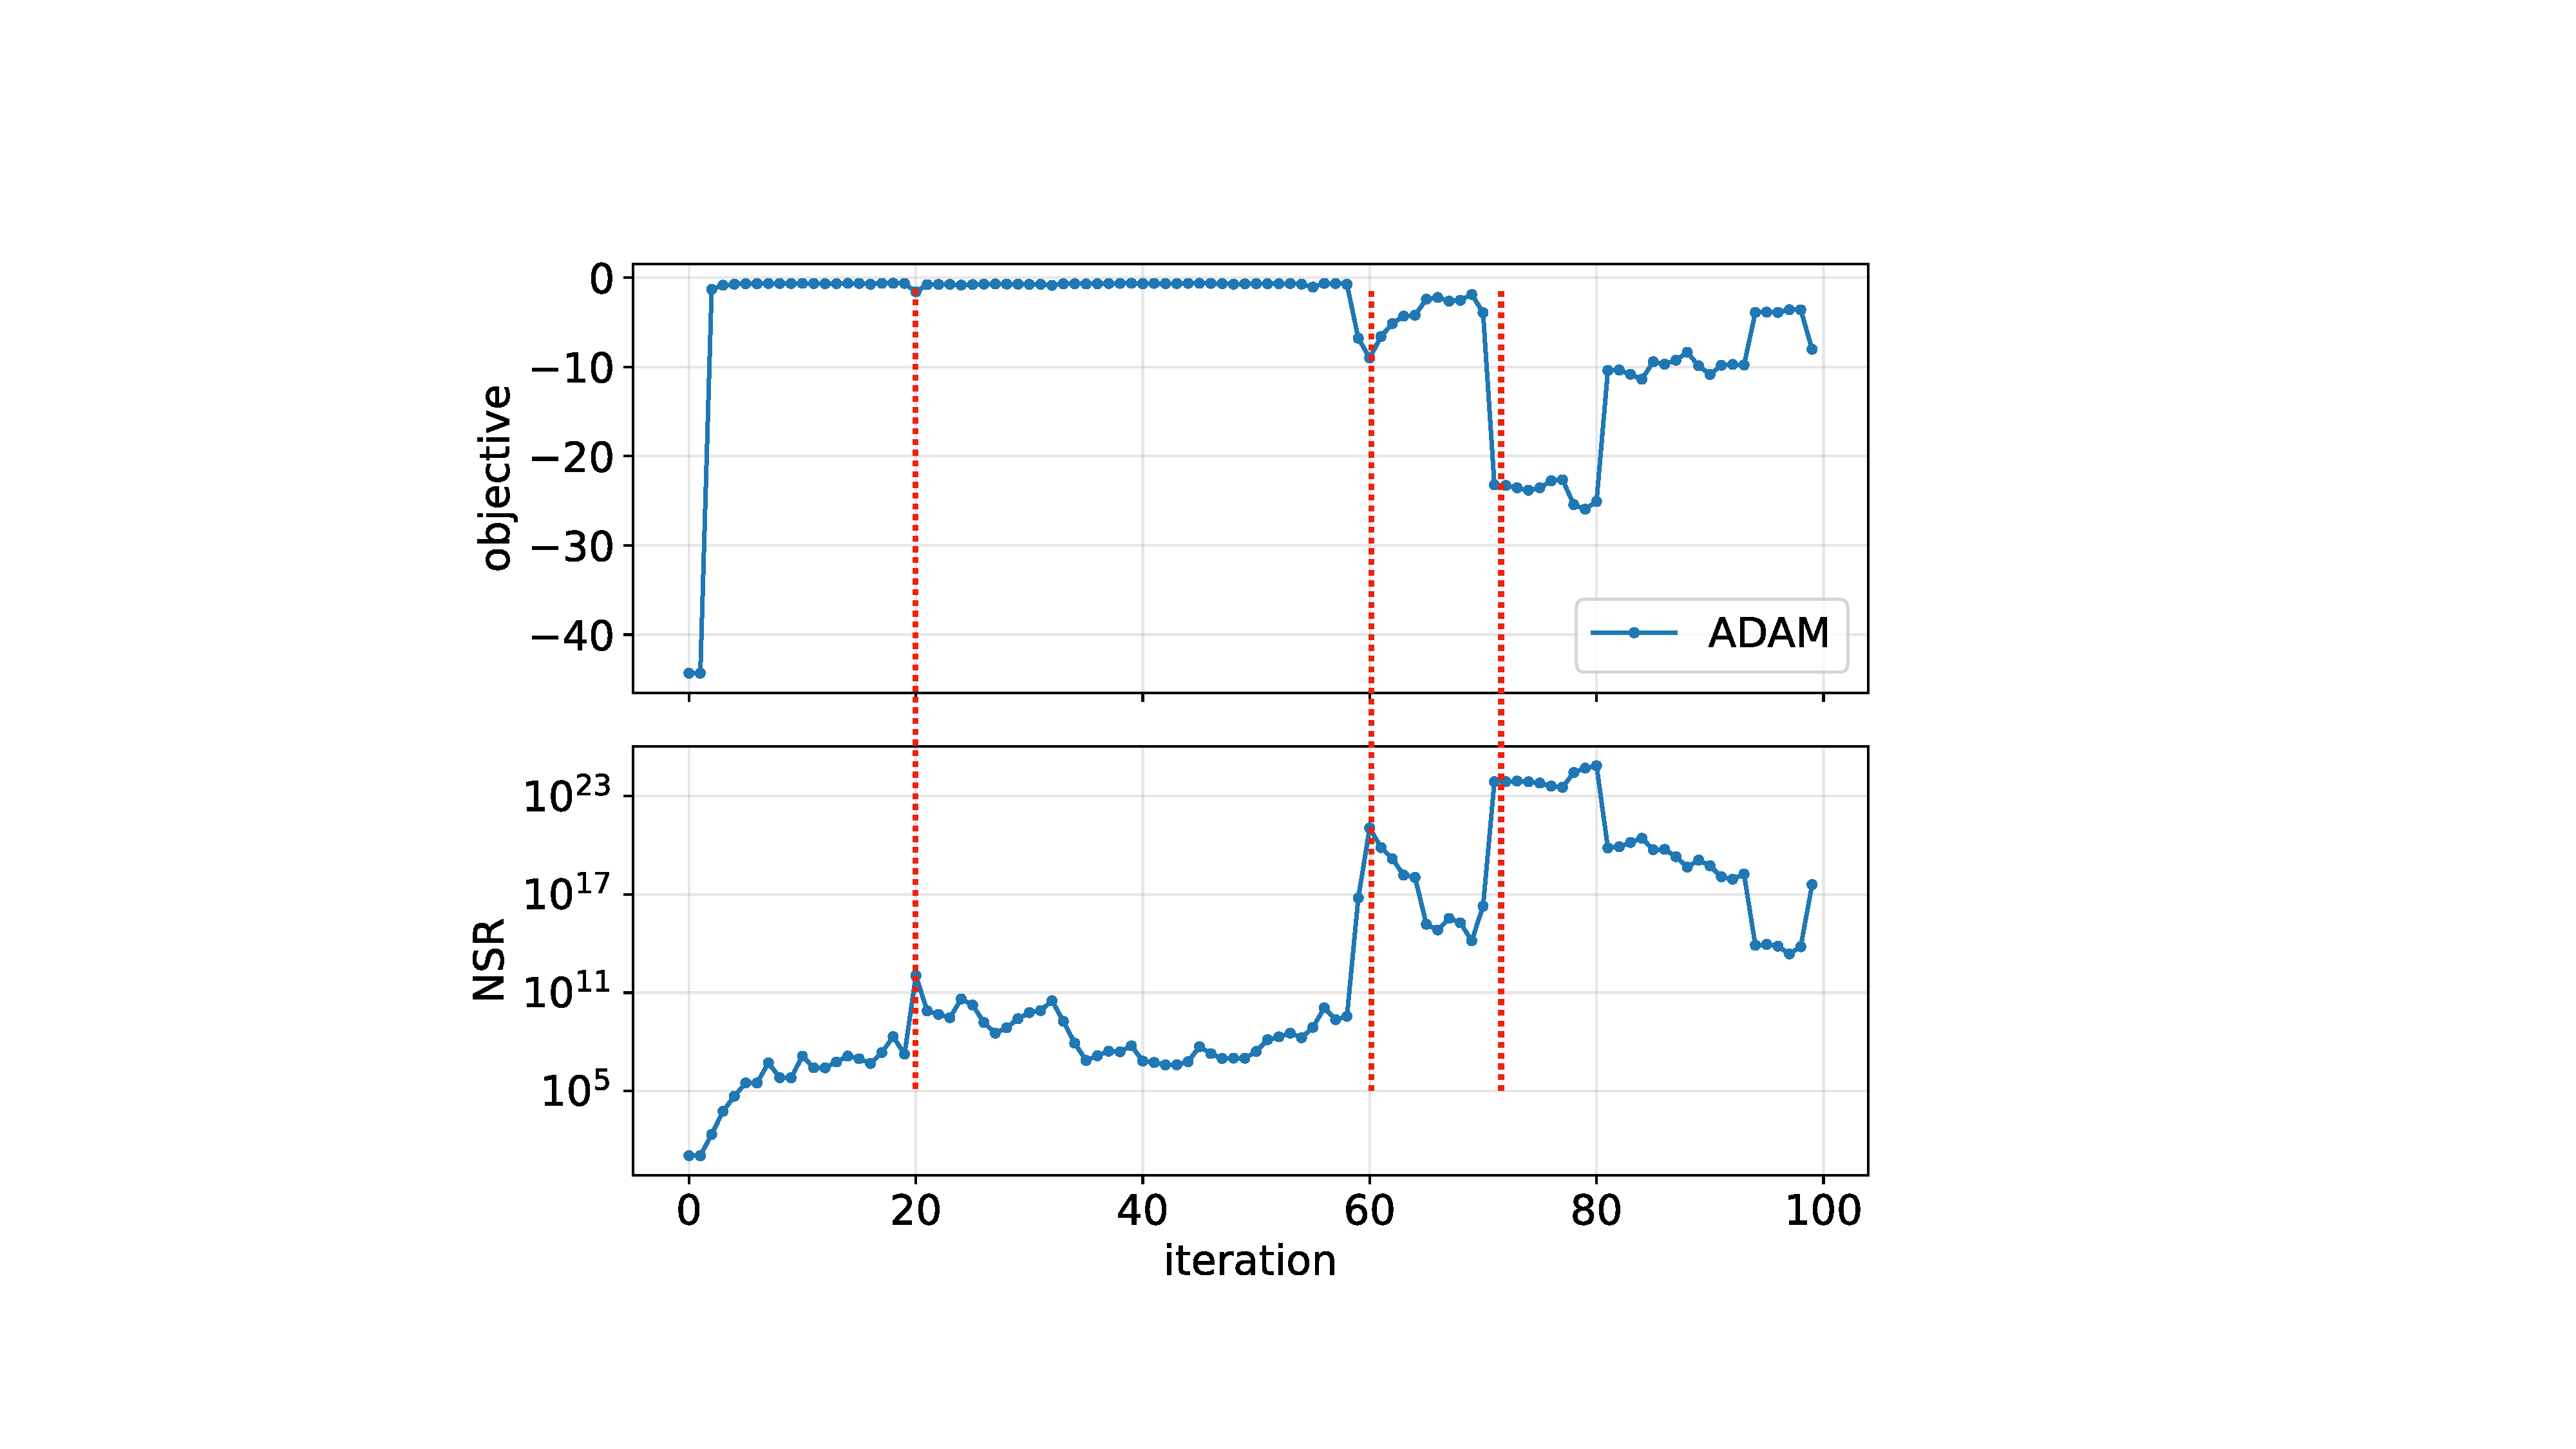
\includegraphics[width=0.36\textwidth]{figure/policy_collapse.pdf}%
  \caption{NSR (bottom) and objective (top) during training on the quadratic system. As the policy oscillates near the optimum, a single inaccurate gradient step triggers policy collapse.}
  \label{fig:policy_collapse}
  \vspace{-4mm}
\end{figure}


% \hy{The following summary may be removed.}

% \textbf{Summary of LQG.} Theorem~\ref{thm:lqg-variance-one-step} and Theorem~\ref{thm:lqr-variance-T-compose} provide exact expressions for both one-step and multi-step PG variance in LQG problems, while Theorem~\ref{thm:lqr-variance-T-bound} and Theorem~\ref{thm:lqr-lifted-state-maps-bound} give interpretable upper bounds that capture the key scaling factors. In particular, small policy covariance \(\Sigma\), large initial-state covariance \(\Sigma_0\), and large spectral radius \(\rho(F)\) of the closed-loop system all contribute to large variance. Numerical experiments confirm these trends, and show that SGD and Adam optimizers can struggle when the NSR becomes large near optimality.
